\section{系统函数与系统特性}

\subsection{系统函数的零、极点分布图}

\begin{BoxDefinition}[零、极点分布图]
    由系统函数定义可知LTI系统是复变量$s$或$z$的有理分式,即
    \begin{Equation}
        H(\cdot) = \frac{B(\cdot)}{A(\cdot)}
    \end{Equation}
    其中$A(\cdot)=0$的根$p_1,p_2,\dots,p_n$称为系统函数的极点。

    $B(\cdot)$的根$\xi_1,\xi_2,\dots,\xi_m$称为系统函数的零点。

    用$\times$表示极点,$\circ$表示零点画在复平面上即可得零、极点分布图。

    Example.
    \begin{Equation}
        H(s) = \frac{2(s+2)}{(s+1)^2(s^2+1)}
    \end{Equation}
    \begin{Figure}[零、极点分布图]
        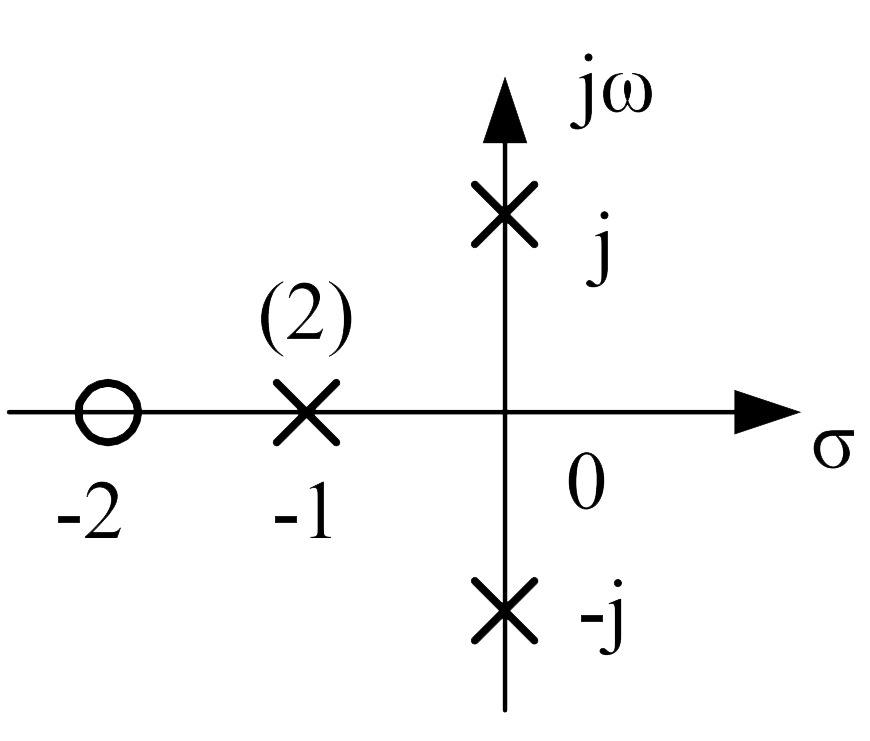
\includegraphics[width=30mm]{img/7.1.png}
    \end{Figure}
\end{BoxDefinition}


\subsection[系统函数与系统的因果性]{系统函数$H(\cdot)$与系统的因果性}

\begin{BoxDefinition}[系统的因果性]*
    因果系统是指系统的零状态响应$y_{zs}(\cdot)$不会出现于$f(\cdot)$之前的系统。

    连续因果系统的充分必要条件是冲激响应满足
    \begin{Equation}
        h(t)=0 \quad t<0
    \end{Equation}
    或者系统函数$H(s)$的收敛域为$\mathrm{Re}\left[s\right]>\sigma_0$

    离散因果系统的充分必要条件是单位响应满足
    \begin{Equation}
        h(k)=0 \quad k<0
    \end{Equation}
    或者系统函数$H(z)$的收敛域为$|z|>\rho_0$
\end{BoxDefinition}

\subsection[系统函数与时域响应]{系统函数$H(\cdot)$与时域响应$h(\cdot)$}

$H(s)$的极点在$s$平面上的位置可分为极点在左半开平面、虚轴和右半开平面三类。

\begin{BoxProperty}[极点在左半开平面的连续因果系统的时域响应]*
    极点在左半开平面时,若系统函数有负实单极点$p=-\alpha(\alpha>0)$,则$A(s)$中有因子$(s+\alpha)$,其所对应的响应函数为
    \begin{Equation}
        h_1(t) = Ke^{-\alpha t}\varepsilon(t)
    \end{Equation}
    若有一对共轭复极点$p_{12}=-\alpha\pm\mathrm{j}\beta$,则$A(s)$中有因子$\left[(s+\alpha)^2+\beta^2\right]$,其所对应的响应函数为
    \begin{Equation}
        h_2(t) = Ke^{-\alpha t}\cos(\beta t+\theta)\varepsilon(t)
    \end{Equation}
    若有$r$重极点,则$A(s)$中有因子$(s+\alpha)^r$或$\left[(s+\alpha)^2+\beta^2\right]^r$,其所对应的响应函数为
    \begin{Equation}
        h_3(t) = K_it_ie^{-\alpha t}\varepsilon(t) \quad (i=0,1,2,\dots,r-1)
    \end{Equation}
    或
    \begin{Equation}
        h_3(t) = K_it^ie^{-\alpha t}\cos(\beta t+\theta)\varepsilon(t) \quad (i=0,1,2,\dots,r-1)
    \end{Equation}
    以上三种情况在$t\rightarrow \infty$时,响应均趋于$0$,为暂态分量,该系统稳定。
\end{BoxProperty}

\begin{BoxProperty}[极点在虚轴上的连续因果系统的时域响应]*
    极点在虚轴上时,若系统函数有负实单极点$p=0$或$p_{12}=\pm\mathrm{j}\beta$,则响应函数为
    \begin{Equation}
        h_1(t) = K\varepsilon(t)
    \end{Equation}
    或
    \begin{Equation}
        h_2(t) = K\cos(\beta t+ \theta)\varepsilon(t)
    \end{Equation}
    此时响应为稳态分量,对应系统稳定。

    若系统函数有$r$重极点,相应$A(s)$中有$s^r$或$(s^2+\beta^2)^r$,其响应函数为
    \begin{Equation}
        h_2(t) = K_i t^i \varepsilon(t) \quad (i=0,1,2,\dots,r-1)
    \end{Equation}
    或
    \begin{Equation}
        h_3(t) = K_i t^i \cos(\beta t+ \theta)\varepsilon(t) \quad (i=0,1,2,\dots,r-1)
    \end{Equation}
    此时响应为递增函数,对应系统不稳定。
\end{BoxProperty}

\begin{BoxProperty}[极点在右半开平面的连续因果系统的时域响应]*
    极点在右半开平面时,其对应的响应函数都是递增的,系统不稳定。
\end{BoxProperty}

由以上性质可知,LTI连续因果系统的$h(t)$函数形式由$H(t)$的极点确定。

\subsection{系统函数与频率响应}

\begin{BoxDefinition}[全通函数]*
    若系统的幅频响应$|H(\mathrm{j}\omega)|$为常数,则称为全通系统,其相应的$H(s)$称为全通函数。

    凡极点位于左半开平面,零点位于右半开平面,并且所有零点与极点相对于虚轴一一镜像对称的系统函数$H(s)$即为全通函数。
\end{BoxDefinition}

\begin{BoxDefinition}[最小相移函数]*
    对于有相同幅频特性的系统函数而言,右半开平面没有零点的系统函数称为最小相移函数。
\end{BoxDefinition}